%% main.tex — Continuous Myhill-Nerode Quotient Learning via Kernel MMD
%% NeurIPS 2024 style (falls back to plain article if neurips_2024.sty unavailable)

\documentclass[10pt]{article}

%% --- NeurIPS 2024 style (use if neurips_2024.sty is available) ---
%% \usepackage[final]{neurips_2024}

%% --- Page geometry approximating NeurIPS 2-column at 10pt ---
\usepackage[margin=1in]{geometry}

%% --- Core packages ---
\usepackage[utf8]{inputenc}
\usepackage[T1]{fontenc}
%\usepackage{microtype}  % disabled: font expansion not available in this TeX install
\usepackage{amsmath, amssymb, amsthm}
\usepackage{mathtools}
\usepackage{bm}
\usepackage{booktabs}
\usepackage{graphicx}
\usepackage{hyperref}
\usepackage{xcolor}
\usepackage{algorithm}
\usepackage{algpseudocode}
\usepackage{natbib}
\usepackage{url}

%% --- Theorem environments ---
\newtheorem{theorem}{Theorem}
\newtheorem{lemma}{Lemma}
\newtheorem{proposition}{Proposition}
\newtheorem{corollary}[theorem]{Corollary}
\newtheorem{definition}{Definition}
\newtheorem{remark}{Remark}

%% --- Math macros ---
\newcommand{\calQ}{\mathcal{Q}}
\newcommand{\calH}{\mathcal{H}}
\newcommand{\calO}{\mathcal{O}}
\newcommand{\calA}{\mathcal{A}}
\newcommand{\calS}{\mathcal{S}}
\newcommand{\calK}{\mathcal{K}}
\newcommand{\calC}{\mathcal{C}}
\newcommand{\calP}{\mathcal{P}}
\newcommand{\calM}{\mathcal{M}}
\newcommand{\calB}{\mathcal{B}}
\newcommand{\bbR}{\mathbb{R}}
\newcommand{\bbE}{\mathbb{E}}
\newcommand{\epsMMD}{\varepsilon_{\mathrm{MMD}}}
\newcommand{\epsmin}{\varepsilon_{\min}}
\newcommand{\Qstar}{\mathcal{Q}^*}
\newcommand{\mmd}{\mathrm{MMD}}
\newcommand{\TV}{\mathrm{TV}}
\newcommand{\RKHS}{\mathcal{H}_k}
\newcommand{\phih}{\phi_h}
\newcommand{\Khist}{K_{\mathrm{hist}}}

%% ============================================================
\begin{document}

\title{Myhill--Nerode Quotient Learning\\
       for Continuous Observation--Action Spaces\\
       via Kernel Maximum Mean Discrepancy}

\author{%
  Anonymous Author(s)\\
  Under Review
}

\maketitle

% ============================================================
\begin{abstract}
% ============================================================
Model-free identification of the minimal world-model of a bounded agent in a
partially observable Markov decision process (POMDP) has been made tractable in
the \emph{finite} setting by Myhill--Nerode quotient learning: a permutation
G-test on fixed-policy continuation histograms clusters histories into
continuation-equivalence classes.  When observations and actions are
continuous the continuation alphabet is infinite and the G-test is undefined.

We extend quotient learning to continuous observation--action spaces
$\calO\times\calA\subseteq\bbR^d$.  Histories are keyed by coarse quantile
bins of the observation stream and, for every pair of bins, the continuation
laws are compared with a kernel maximum mean discrepancy (MMD) permutation test
on raw continuation vectors under Benjamini--Hochberg control; bins whose test
does not reject are merged by union--find.  We (i) identify the estimator's
target precisely---the \emph{bin-level} continuation quotient---and give
conditions under which it coincides with the latent quotient of index $n$;
(ii) prove an alphabet-free trajectory bound
$N=O\!\big(\Khist(\tau{+}k)\log(\Khist/\delta)/(T\epsMMD^2)\big)$, with
$\Khist=O(n)$ active bins, in which the alphabet size $|\calC|$ of the finite
bound is replaced by the MMD separation $\epsMMD$ (dimension enters only
through $\epsMMD$); and (iii) characterise the finite-sample behaviour as a
\emph{resolution} effect: distinctions below the test's detection scale are
merged, so the returned quotient size depends on the bin count $B$ and on the
per-test sample budget.

Empirically, at the natural resolution ($B{=}n$ aligned bins, or $B$ chosen
by silhouette auto-selection) the estimator returns the latent index on 90/90
runs across Tiger ($\sigma{=}0.5$), K-cycle ($K\le16$) and a Gaussian-mixture
random walk, while G-test, Wasserstein-threshold and DBC baselines fail on
K-cycle; over-provisioning $B{=}2K$ mis-estimates the index for $K\ge3$
(over-splitting up to $2K$, and chaining-induced under-splitting at $K{=}16$),
as the resolution analysis predicts.  On PO-MuJoCo the estimator returns $\hat n{=}B$
(all bin pairs separable) with classes that are strongly return-stratified.
On a 4-state chain Dec-POMDP the estimated critical communication rate
$\hat R_{\rm crit}=H(\hat Q_A\mid\hat Q_B)$ tracks the analytical value within
$0.8\%$ mean error whenever both agents' quotients are non-trivial; on
Dec-Tiger the estimate is accurate on the seeds where agent A recovers two
classes but agent-A over-splitting (which inflates the conditional entropy)
occurs on 5/10 seeds at $\alpha{=}0.05$.  We report all seeds and discuss the
limitations candidly.
\end{abstract}

% ============================================================
\section{Introduction}
% ============================================================

A fundamental question in reinforcement learning is: \emph{how much of the
world does a bounded agent need to model?}  For agents acting under partial
observability, a natural answer is the \emph{Myhill--Nerode quotient} of the
history space under a fixed behaviour policy: two histories are equivalent if
they induce the same distribution over futures.  \citet{nixon2026quotient}
develops this theory for bounded agents and \citet{nixon2026rcrit} uses the
resulting quotient to define a \emph{critical communication rate}
$R_{\rm crit}$ for multi-agent coordination.  A companion paper
\citep{Companion2026} gives a model-free estimator for \emph{finite}
observation--action alphabets: a permutation G-test on continuation histograms
decides, for each pair of observed histories, whether their $k$-step
continuation distributions differ, and a union--find pass merges the pairs that
do not; the required number of trajectories is
$N=O(|\calC|\,n^2k\tau\log(n/\delta)/(T\epsmin^2))$ where $|\calC|$ is the
continuation alphabet.

\paragraph{The gap: continuous spaces.}
Real POMDPs---manipulation, locomotion, audition---have continuous observation
and action spaces.  Applying the finite estimator requires discretising
$\calO\times\calA$ into an alphabet $\calC$, which (1) makes $|\calC|$ grow
exponentially in the dimension and (2) conflates continuation distributions
that differ only within a cell.  Both pathologies are visible in our
experiments: a 3-bin G-test never recovers the two Tiger classes and an 8-bin
G-test over-splits the 4-state K-cycle into 8 classes (Table~\ref{tab:ablation}).

\paragraph{Our contribution.}
We replace the G-test with a kernel MMD permutation test on raw continuation
vectors \citep{Gretton2012}, so no discretisation of the continuation space is
needed, and key histories by coarse quantile bins so that enough continuations
accumulate per key.  Concretely:
\begin{enumerate}
\item \textbf{Algorithm (Section~\ref{sec:method}).}  Quantile binning of the
  observation stream into $B$ bins, a biased-MMD$^2$ permutation test with a
  median-heuristic RBF kernel for every pair of bins, Benjamini--Hochberg (BH)
  control over pairs, and union--find merging.
\item \textbf{What is estimated (Section~\ref{sec:method}).}  In continuous
  spaces the exact continuation-equivalence quotient of the \emph{history}
  space is generically infinite (every observation value induces a different
  posterior), so we define the estimator's target as the \emph{bin-level}
  quotient $\Qstar_B$---the partition of the $B$ bins by equality of their
  bin-conditional continuation laws---and give conditions (bounded-support
  noise, bin edges aligned with class boundaries) under which
  $|\Qstar_B|$ equals the latent index $n$
  (Proposition~\ref{prop:binning}).
\item \textbf{Alphabet-free sample complexity (Section~\ref{sec:theory}).}
  Using the concentration of the biased MMD statistic
  \citep[Thm.~7, Cor.~9]{Gretton2012} we prove that
  $N=O(\Khist(\tau{+}k)\log(\Khist/\delta)/(T\epsMMD^2))$ trajectories suffice
  to recover $\Qstar_B$ with probability $1-\delta$, where $\Khist\le B^\ell$
  is the number of active history bins ($\Khist=B=O(n)$ in all our
  experiments).  The $|\calC|$ factor of the finite bound disappears; the
  dimension enters only through $\epsMMD$.
\item \textbf{Resolution analysis.}  Because a two-sample test with $m$
  samples cannot detect MMD gaps below $\approx\sqrt{\log(1/\alpha)/m}$, the
  finite-sample estimate is the quotient at that resolution: same-class bins
  whose laws differ slightly are merged, and distinct latent classes are
  separated only if their gap exceeds the detection scale.  This explains all
  of our empirical findings, including the successes (aligned $B{=}n$) and the
  failures (over- and under-splitting at $B{=}2K$).
\item \textbf{Experiments (Section~\ref{sec:experiments}).}  Ground-truth
  recovery on Tiger, K-cycle and a Gaussian-mixture random walk (90/90 at
  $B{=}n$), sensitivity to $B$ and $N$, an ablation against G-test,
  Wasserstein-threshold and DBC baselines, PO-MuJoCo (HalfCheetah, Ant), and
  end-to-end $R_{\rm crit}$ estimation on Dec-Tiger and a 4-state chain
  Dec-POMDP.  All numbers are computed from the result files shipped with the
  code and every seed is reported.
\end{enumerate}

\paragraph{Paper organisation.}
Section~\ref{sec:related} surveys related work; Section~\ref{sec:method}
defines the target and the algorithm; Section~\ref{sec:theory} states the
guarantees; Section~\ref{sec:experiments} presents experiments;
Section~\ref{sec:limitations} discusses limitations; Section~\ref{sec:conclusion}
concludes.  Proofs and full experimental specifications are in the supplement.

% ============================================================
\section{Related Work}
\label{sec:related}
% ============================================================

\paragraph{PAC learning in POMDPs.}
Observable operator models \citep{Jaeger2000}, spectral methods for predictive state representations \citep{Boots2011} and
tensor methods \citep{Azizzadenesheli2016} estimate latent dynamics with
sample-efficiency guarantees when the number of latent states (or Hankel rank)
is known.  Our approach is model-free and targets only the quotient partition.

\paragraph{Bisimulation and state abstraction.}
Bisimulation relations \citep{Larsen1991} and bisimulation metrics
\citep{Ferns2004,Castro2020} formalise (approximate) behavioural equivalence of
MDP states; \citet{Castro2009} extend these relations to partially observable
MDPs.  The brittleness of exact equivalence under perturbation is the classical
motivation for metrics \citep{Ferns2004}.  Deep Bisimulation for Control (DBC)
\citep{Zhang2020} learns metric-respecting representations.  \citet{Abel2020}
analyse approximate state abstractions and their value loss.  Our object is
different: we cluster \emph{observed histories} under a fixed policy, we output
a discrete partition (which is what the $R_{\rm crit}$ theory of
\citet{nixon2026rcrit} consumes), and---in line with the bisimulation-metric
literature---we make explicit that in continuous spaces the exact partition is
generically infinite and what is recovered is a partition at a resolution set
by the binning and the test.

\paragraph{Policy dependence.}
The estimated quotient is the fixed-policy continuation-equivalence partition;
under a random policy it may be trivial ($n{=}1$) and under a structured policy
non-trivial.  This is by design: the quotient characterises the agent's minimal
perception \emph{relative to its behaviour policy} \citep{nixon2026quotient}.

\paragraph{Two-sample kernel testing.}
The MMD \citep{Gretton2012} is a nonparametric two-sample statistic that is
consistent against all alternatives for characteristic kernels; permutation
calibration gives exact finite-sample level.  Block estimators
\citep{Zaremba2013} trade variance for $O(m)$ cost; we use the biased
$O(m^2)$ estimator with at most $m_{\max}=300$ samples per side.
\citet{Ramdas2015} show that with a fixed (e.g.\ median-heuristic) kernel the
MMD separation between fixed alternatives typically \emph{decreases} with
dimension; this is why our bound is ``alphabet-free'' rather than
``dimension-free'' (Remark~\ref{rem:dimension}).

% ============================================================
\section{Method}
\label{sec:method}
% ============================================================

\subsection{Problem Formulation}

\begin{definition}[Continuous POMDP]
A continuous POMDP is a tuple $(\calS,\calO,\calA,T,R,\Omega,\gamma)$ with
$\calO\subseteq\bbR^{d_O}$, $\calA\subseteq\bbR^{d_A}$ (or a finite set),
transition kernel $T:\calS\times\calA\to\Delta(\calS)$, emission kernel
$\Omega:\calS\to\Delta(\calO)$, reward $R$ and discount $\gamma$.
\end{definition}

\begin{definition}[Continuation law]
Fix a behaviour policy $\pi$ and a window $k\ge1$.  For a history
$h=(o_1,a_1,\dots,o_t)$ the \emph{$k$-step continuation law}
$P^{(k)}_{h,\pi}$ is the law of $c=(o_{t+1},a_{t+1},\dots,o_{t+k})\in\bbR^{d_c}$,
$d_c=k\,d_O+(k{-}1)d_A$, obtained by executing $\pi$ from $h$.
\end{definition}

\begin{definition}[Continuation-equivalence quotient]
$h_1\sim_{\pi,k}h_2$ iff $P^{(k)}_{h_1,\pi}=P^{(k)}_{h_2,\pi}$.  The quotient
$\Qstar_{\pi,k}=\calH/{\sim_{\pi,k}}$ has index $n=|\Qstar_{\pi,k}|$.  We say
the POMDP has \emph{finite latent index $n$} if there is a class map
$c:\calH\to[n]$ with $P^{(k)}_{h,\pi}=P^{(k)}_{c(h)}$.
\end{definition}

\begin{remark}[Exact quotients are generically infinite in continuous spaces]
\label{rem:infinite}
If the emission kernel has a density with unbounded support (e.g.\ Gaussian
noise), the posterior over the latent state given a history varies
continuously with the observed values, and so does the continuation law; hence
$\Qstar_{\pi,k}$ is uncountable and the latent index is not the history
quotient index.  For instance, in Tiger with $o=\pm1+\mathcal N(0,\sigma^2)$
and one-step histories, $P(\text{Right}\mid o)=\mathrm{logistic}(2o/\sigma^2)$
and no two observation values share a continuation law.  What a finite
estimator can target is a quotient at a \emph{resolution}, which we now define.
\end{remark}

\subsection{Coarse History Binning and the Bin-Level Quotient}
\label{sec:binning}

Given $N$ trajectories we reduce each observation to a scalar
$z(o)$ ($z(o)=o$ if $d_O=1$, else $z(o)=\|o\|_2$; the implementation exposes
this map), fit $B$ equal-frequency (quantile) edges of $z$ over all time
steps, and key a history of length $\ell$ by the tuple of bin indices of its
last $\ell$ observations (and, when actions are discrete, the interleaved
actions).  All experiments use $\ell=1$, so a key is a single bin.  Let
$\calB$ be the set of active keys ($\Khist=|\calB|\le B^\ell$) and, for
$b\in\calB$, let $P_b$ be the \emph{bin-conditional continuation law}: the law
of $c$ given that the history falls in $b$ (a mixture of $P^{(k)}_{h,\pi}$
over $h\in b$).

\begin{definition}[Bin-level quotient]
$\Qstar_B$ is the partition of $\calB$ induced by $b\sim b'\iff P_b=P_{b'}$.
The estimator's target is $\Qstar_B$; we write $\hat\calQ_B$ for its output.
\end{definition}

$\Qstar_B$ is always finite.  It coincides with the latent class partition
(so $|\Qstar_B|=n$) exactly when every bin is \emph{pure}, i.e.\ contains
histories of a single latent class (Proposition~\ref{prop:binning}).  Under
Gaussian noise no bin is exactly pure and $\Qstar_B$ generically has $\Khist$
classes; the estimator then returns a coarsening determined by the detection
scale of the test (Remark~\ref{rem:resolution}).  In practice $B$ is set to
the number of clusters in the observation marginal (Algorithm~2 in the
supplement selects it by silhouette score) or from domain knowledge.

\subsection{Kernel MMD Test}
\label{sec:mmd}

For each pair $(b_1,b_2)$ we take up to $m_{\max}$ continuation vectors from
each bin (deterministically subsampled per pair) and test $H_0:P_{b_1}=P_{b_2}$
with the biased MMD$^2$ statistic
\begin{equation}
\widehat{\mmd}^2
  = \frac{1}{m_1^2}\sum_{i,j}\kappa(c^{(1)}_i,c^{(1)}_j)
  + \frac{1}{m_2^2}\sum_{i,j}\kappa(c^{(2)}_i,c^{(2)}_j)
  - \frac{2}{m_1m_2}\sum_{i,j}\kappa(c^{(1)}_i,c^{(2)}_j),
\label{eq:mmd}
\end{equation}
where $\kappa(x,y)=\exp(-\|x-y\|^2/(2\sigma^2))$ and the bandwidth follows
the median heuristic $2\sigma^2=\mathrm{median}\{\|x-y\|^2\}$ over the pooled
sample (so $\kappa(x,y)=\exp(-\|x-y\|^2/\mathrm{med})$).  Significance is
assessed by $R$ random permutations of the pooled sample,
$p=(1+\#\{\text{perm.\ statistic}\ge\text{observed}\})/(R+1)$, which is
exact-level for exchangeable samples.  Because the smallest attainable
$p$-value is $1/(R{+}1)$, per-pair Bonferroni levels $\alpha/\Khist^2$ are
unattainable at moderate $R$; we therefore apply Benjamini--Hochberg \citep{Benjamini1995} at level
$\alpha$ over all $\binom{\Khist}{2}$ pairs and declare a pair \emph{different}
iff its $p$-value is at or below the BH threshold.  BH controls the false
discovery rate of \emph{splits}; missed splits (Type~II errors) are governed by
power, and a single missed split between two classes merges them entirely
under union--find, so the conservative failure mode of the estimator is
under-splitting at small $m$ and over-splitting at large $m$ (Section~\ref{sec:theory}).

\subsection{Union--Find Quotient Estimator}

Bins are merged whenever the test does \emph{not} reject; the resulting
single-linkage partition is $\hat\calQ_B$.  Algorithm~\ref{alg:cqe} states the
procedure as implemented.  For the analysis we also consider variant~(T), in
which step~5 uses the analytic threshold of \citet[Cor.~9]{Gretton2012} at a
per-pair level $\alpha_0$; variant~(T) is the object of Theorem~\ref{thm:main}.

\begin{algorithm}[t]
\caption{\textsc{ContinuousQuotientEstimator}}
\label{alg:cqe}
\begin{algorithmic}[1]
\Require Trajectories $\{(o^{(i)}_1,a^{(i)}_1,\dots,o^{(i)}_T)\}_{i=1}^N$,
         history length $\ell$, window $k$, bins $B$, minimum count $m_{\min}$,
         cap $m_{\max}$, level $\alpha$, permutations $R$.
\Ensure  Partition $\hat\calQ_B$ of active keys.
\State \textbf{Quantile edges.}  Fit $B$ equal-frequency edges of $z(o)$ over all $(i,t)$.
\State \textbf{Key histories.}  For each $(i,t)$ compute the key $b^{(i)}_t$ from the
       binned last $\ell$ observations (and discrete actions).
\State \textbf{Accumulate continuations.}  $\calC_b\leftarrow\{(o^{(i)}_{t+1:t+k},a^{(i)}_{t+1:t+k-1}):b^{(i)}_t=b\}$;
       keep keys with $|\calC_b|\ge m_{\min}$; $\Khist\leftarrow$ number of kept keys.
\State \textbf{MMD tests.}  For each pair $b_1<b_2$: subsample at most $m_{\max}$ vectors per side,
       compute \eqref{eq:mmd} with the median-heuristic bandwidth and the permutation $p$-value.
\State \textbf{Multiplicity.}  Apply BH at level $\alpha$ to all $p$-values; reject $=$ ``different''.
\State \textbf{Union--find.}  Merge every non-rejected pair; \Return $\hat\calQ_B$.
\end{algorithmic}
\end{algorithm}

% ============================================================
\section{Theoretical Analysis}
\label{sec:theory}
% ============================================================

Throughout, $\kappa^2=\sup_x\kappa(x,x)$ ($\kappa=1$ for the RBF kernel).

\begin{lemma}[MMD is dominated by total variation]
\label{lem:tv}
For any bounded kernel and any $P,Q$, $\mmd(P,Q)\le2\kappa\,\TV(P,Q)$.
Consequently, if $h\mapsto P^{(k)}_{h,\pi}$ is $L$-Lipschitz in TV with respect
to the sup-norm on histories and bin $b$ has diameter $w_b$ in observation
space, then $\mmd(P^{(k)}_{h,\pi},P_b)\le2\kappa Lw_b$ for every $h\in b$.
\end{lemma}

Lemma~\ref{lem:tv} bounds the \emph{within-bin heterogeneity} of continuation
laws (proof in the supplement).  Note that the relevant width is the bin's
diameter in observation space, not $1/B$.

\begin{theorem}[Recovery of the bin-level quotient]
\label{thm:main}
Let $\epsMMD=\min\{\mmd(P_b,P_{b'}):b,b'\in\calB,\ P_b\ne P_{b'}\}>0$.
Suppose each active bin supplies $m$ i.i.d.\ continuation samples and run
Algorithm~\ref{alg:cqe}, variant~(T), with per-pair level
$\alpha_0=\delta/\Khist^2$.  If
\begin{equation}
  m\;\ge\;\frac{16\kappa^2}{\epsMMD^2}\Big(8+\log\frac{2\Khist^4}{\delta^2}\Big)
  \;=\;O\!\Big(\frac{\log(\Khist/\delta)}{\epsMMD^2}\Big),
  \label{eq:m-bound}
\end{equation}
then $\hat\calQ_B=\Qstar_B$ with probability at least $1-\delta$.
If, in addition, the process is $\tau$-mixing so that from $N$ trajectories of
length $T$ every active bin yields at least
$m\ge N(T{-}\ell{-}k{+}1)/(c\,\Khist(\tau{+}k))$ effectively independent
continuation samples ($c$ an absolute constant; quantile bins have equal mass),
then it suffices that
\begin{equation}
  N \;=\; O\!\left(\frac{\Khist\,(\tau+k)\,\log(\Khist/\delta)}{T\,\epsMMD^2}\right).
  \label{eq:bound}
\end{equation}
\end{theorem}

The proof (supplement, Section~A) combines the deviation bound for the biased
MMD statistic \citep[Thm.~7]{Gretton2012}, the null threshold of
\citet[Cor.~9]{Gretton2012}, and a union bound over the at most $\Khist^2/2$
pairs; the constants are explicit.  With $\ell=1$ and $B=O(n)$ bins,
$\Khist=B=O(n)$ and \eqref{eq:bound} reads
$O(n(\tau{+}k)\log(n/\delta)/(T\epsMMD^2))$.

\paragraph{Discussion.}
Compared with the finite-alphabet bound
$O(|\calC|n^2k\tau\log(n/\delta)/(T\epsmin^2))$ of the companion paper, the
$|\calC|$ factor is gone: the biased MMD deviates from its population value by
$O(\kappa/\sqrt m)$ regardless of $d_c$ or of any alphabet
\citep[Thm.~7]{Gretton2012}.  One factor of $n$ is also absent because quantile
bins have equal mass by construction, so no term is needed to guarantee that
every history is observed often enough.  The remaining dependence on $\Khist$
is linear and comes from spreading the $NT$ samples over the bins.

\begin{remark}[Dimension enters through $\epsMMD$]
\label{rem:dimension}
Bound \eqref{eq:bound} has no explicit dependence on $d_c$, but $\epsMMD$
does: for a fixed alternative and a median-heuristic RBF kernel the MMD
separation typically shrinks as $d_c$ grows \citep{Ramdas2015}.  The bound
should therefore be read as \emph{alphabet-free}, not as a claim that
continuous quotient learning is easy in high dimension.
\end{remark}

\begin{remark}[Permutation calibration and BH]
Theorem~\ref{thm:main} is stated for the analytic threshold.  The permutation
test used in Algorithm~\ref{alg:cqe} is exact-level and asymptotically
equivalent \citep[\S8]{Gretton2012}, but with $R$ permutations no $p$-value is
below $1/(R{+}1)$; family-wise control at $\alpha/\Khist^2$ would need
$R\ge\Khist^2/\alpha$.  BH at level $\alpha$ is what we run; it controls the
false-discovery rate of splits rather than the family-wise error, and its
threshold is at least as liberal as Bonferroni's.
\end{remark}

\begin{proposition}[When the bin-level quotient equals the latent quotient]
\label{prop:binning}
Assume finite latent index $n$ with class map $c$, one-step keys ($\ell=1$),
and let $F$ be the marginal CDF of the binning scalar $z$.
\begin{enumerate}
\item[(a)] \emph{Separated supports.}  The supports of $z$ under the $n$
  classes are intervals $I_1<\dots<I_n$ with gaps between consecutive intervals.
\item[(b)] \emph{Alignment.}  For every $i<n$, $F(\sup I_i)$ is a multiple of $1/B$.
\end{enumerate}
Under (a) and (b), with probability $\to1$ as $N\to\infty$ every non-empty
bin is pure, $\Qstar_B$ is the class partition ($|\Qstar_B|=n$), and
Algorithm~\ref{alg:cqe} variant~(T) with $\alpha_0=\alpha_N\to0$,
$\log(1/\alpha_N)/m_N\to0$ returns it with probability $\to1$.
Under (a) alone, at most $n-1$ bins straddle a class boundary; each is a
proper two-component mixture of neighbouring class laws, so
$n\le|\Qstar_B|\le2n-1$ and the same conclusion holds for $\Qstar_B$.
\end{proposition}

The proof is in the supplement (Section~B).  Condition~(b) holds for the
K-cycle and Gaussian-mixture environments with $B=n$ (equal class masses) and
for Tiger with any even $B$ (symmetric marginal); it fails for generic
$B>n$, which is why over-provisioning $B$ can create extra classes.
Condition~(a) does \emph{not} hold for Gaussian noise; the corrected version
of the earlier ``sub-Gaussian $3\sigma<\Delta/2$'' statement is that the
cross-contamination fraction of a boundary bin converges to a \emph{positive}
constant, so the boundary bin's law is a permanent mixture and would eventually
be split by a consistent test.

\begin{remark}[Resolution and the sample cap]
\label{rem:resolution}
With $m$ samples per side and level $\alpha$, the null threshold is
$t_\alpha=\sqrt{2\kappa^2/m}\,(1+\sqrt{2\log(1/\alpha)})$ \citep[Cor.~9]{Gretton2012};
pairs whose MMD gap is well below $t_\alpha$ are (with high probability)
merged and pairs whose gap exceeds $\approx t_\alpha+4\kappa/\sqrt m$ are split.
Hence the finite-sample output is the quotient of $\calB$ at resolution
$\approx t_\alpha$.  Because Algorithm~\ref{alg:cqe} caps each side at
$m_{\max}$ (300 in all experiments) the resolution does \emph{not} sharpen
indefinitely with $N$; this is why, in Gaussian-noise environments, the
estimator returns the latent index stably across $N$ at $B=n$
(within-class bin gaps stay below $t_\alpha$) while returning up to $B$
classes when $B$ is over-provisioned (Table~\ref{tab:sensitivity}).
Combined with Lemma~\ref{lem:tv}, the latent index is returned whenever
$2\kappa Lw_{\max}\ll t_\alpha\ll\epsMMD^{\rm latent}$, where
$\epsMMD^{\rm latent}$ is the smallest gap between distinct latent class laws.
\end{remark}

% ============================================================
\section{Experiments}
\label{sec:experiments}
% ============================================================

All configurations, seeds and result files are listed in the supplement
(Section~C) and shipped with the code; unless stated otherwise
$\ell=1$, $k=2$, $m_{\min}=20$, $m_{\max}=300$, RBF kernel with the median
heuristic, and BH correction.

\subsection{Environments}

\paragraph{Tiger (Gaussian observations).}
The classic Tiger POMDP \citep{Kaelbling1998}: two hidden states, three discrete actions (listen, open-left, open-right; an
open action re-draws the state uniformly), scalar observation
$o=\pm1+\mathcal N(0,\sigma^2)$ with $\sigma=0.5$, uniform-random policy,
$T=20$, $B=8$, $\alpha=0.01$, $R=199$.  Latent index $n=2$.

\paragraph{Continuous K-cycle.}
$K\in\{2,3,4,5,8,16\}$ latent phases advanced deterministically,
$o=s/K+\mathcal N(0,0.1^2)$ (equally spaced means, heavy overlap for large
$K$: adjacent means are $1.25\sigma$ apart at $K=8$), single null action,
$T=50$, $N=3000$ ($5000$ for $K=16$), $B=K$, $\alpha=0.01$, $R=199$.  Latent
index $n=K$.

\paragraph{Gaussian-mixture random walk.}
$N_s\in\{3,4,5,6\}$ states, $s'=\mathrm{clip}(s+\delta,0,N_s{-}1)$ with
$\delta\sim\mathrm{Unif}\{-1,0,1\}$ (uniform stationary law),
$o=s+\mathcal N(0,0.15^2)$, $T=50$, $N=2000$, $\alpha=0.01$, $R=99$; run with
$B=N_s$ and with $B$ auto-selected by silhouette.  Latent index $n=N_s$
(boundary states have two successors, interior states three).

\paragraph{PO-HalfCheetah / PO-Ant.}
Gymnasium \texttt{HalfCheetah-v4} (17-dim observation; we zero the 8 joint
positions and the root-$x$ velocity, keeping 8 velocity coordinates) and
\texttt{Ant-v4} (27-dim observation; we keep the 14 velocity coordinates),
zero-torque (passive) policy, plus HalfCheetah under a sinusoidal locomotion
policy; $N=5000$, $T=50$, $B=8$ (or auto), $\alpha=0.05$, $R=99$.  No
ground-truth index exists; see Section~\ref{sec:mujoco}.

\paragraph{Dec-Tiger and 4-state chain Dec-POMDPs.}
Two agents observe the same latent state through independent Gaussian
channels ($\sigma_A,\sigma_B$); listen-only policy; $N=1000$, $T=20$, $B=4$,
$m_{\min}=10$, $\alpha=0.05$, $R=99$.  Dec-Tiger: $o^i=\pm1+\mathcal N(0,\sigma_i^2)$.
Chain: 4-state random walk, $o^i=s/4+\mathcal N(0,\sigma_i^2)$.  For each
agent we fit a quotient, label every step by its class, and compute the plug-in
$\hat R_{\rm crit}=H(\hat Q_A\mid\hat Q_B)$; the analytical value
$H(Q_A\mid Q_B)$ uses the sign/interval classification of the noiseless bin
structure (supplement, Section~C.5).  We use $H(Q_A\mid Q_B)$ as a proxy for
the $R_{\rm crit}$ of \citet{nixon2026rcrit}; the two coincide when
observations are conditionally independent given the state.

\subsection{Baselines}
\textbf{G-test $3$/$8$-bin} (finite estimator of the companion paper after
quantile discretisation of the continuation), \textbf{Wasserstein-$\varepsilon$}
(merge bins whose empirical continuation laws are within $W_1$-distance
$\varepsilon\in\{0.1,0.2,0.5,1.0\}$), and \textbf{DBC} \citep{Zhang2020}
(MLP encoder trained with the bisimulation loss, quotient extracted by
$k$-means with silhouette selection).  All baselines see the same trajectories.

\subsection{Ground-truth recovery at the aligned resolution}

\begin{table}[t]
\centering
\caption{Recovery of the latent index at the aligned resolution $B=n$.
  $\bar n\pm$std over seeds; ``Correct'' counts seeds with $\hat n=n$.
  For GaussMix the silhouette auto-selection chose $B=N_s$ on every seed and
  gave identical results.  Note that with $B=n$ the estimator cannot return
  more than $n$ classes, so this table certifies the absence of spurious
  merges only; Table~\ref{tab:sensitivity} probes over-splitting.}
\label{tab:layer1}
\begin{tabular}{lrrcr}
\toprule
Environment & $N$ & Seeds & $\bar n\pm$std & Correct \\
\midrule
Tiger ($\sigma{=}0.5$, $B{=}8$) & 3000 & 10 & $2.00\pm0.00$ & 10/10 \\
K-cycle $K{=}2$   & 3000 & 10 & $2.00\pm0.00$  & 10/10 \\
K-cycle $K{=}3$   & 3000 & 10 & $3.00\pm0.00$  & 10/10 \\
K-cycle $K{=}4$   & 3000 & 10 & $4.00\pm0.00$  & 10/10 \\
K-cycle $K{=}5$   & 3000 & 10 & $5.00\pm0.00$  & 10/10 \\
K-cycle $K{=}8$   & 3000 & 10 & $8.00\pm0.00$  & 10/10 \\
K-cycle $K{=}16$  & 5000 & 10 & $16.00\pm0.00$ & 10/10 \\
GaussMix $N_s{=}3$ & 2000 & 5 & $3.00\pm0.00$ & 5/5 \\
GaussMix $N_s{=}4$ & 2000 & 5 & $4.00\pm0.00$ & 5/5 \\
GaussMix $N_s{=}5$ & 2000 & 5 & $5.00\pm0.00$ & 5/5 \\
GaussMix $N_s{=}6$ & 2000 & 5 & $6.00\pm0.00$ & 5/5 \\
\bottomrule
\end{tabular}
\end{table}

Table~\ref{tab:layer1} shows exact recovery on all 90 runs when $B$ equals
the latent index (Tiger uses $B=8>n$, which is safe because the same-side
bins have posteriors that differ by less than the detection scale at
$m_{\max}=300$; see below).  Tiger is also correct on 3/3 seeds at every
$N\in\{500,1000,2000,5000\}$ in the ablation runs.

\subsection{Sensitivity to $B$ and $N$}

\begin{table}[t]
\centering
\caption{Resolution effects.  Left: K-cycle with over-provisioned $B=2K$
  ($5$ seeds; $N$ as in Table~\ref{tab:layer1}).  Right: Tiger with $B=8$ as
  $N$ grows ($5$ seeds).  Over-provisioning $B$ produces extra classes for
  $3\le K\le8$ (adjacent half-class bins have detectably different posteriors)
  and chaining-induced under-splitting at $K=16$, whereas at fixed $B$ the
  output is stable in $N$ because the per-test cap $m_{\max}=300$ fixes the
  detection scale.}
\label{tab:sensitivity}
\begin{tabular}{lcc@{\qquad}lcc}
\toprule
K-cycle & $B$ & $\hat n$ (per seed) & Tiger & $N$ & $\hat n$ (per seed) \\
\midrule
$K{=}2$  & 4  & 2, 2, 2, 2, 2 & $B{=}8$ & 1000  & 2, 2, 2, 2, 2 \\
$K{=}3$  & 6  & 3, 4, 3, 4, 4 & $B{=}8$ & 3000  & 2, 2, 2, 2, 2 \\
$K{=}4$  & 8  & 8, 8, 8, 8, 8 & $B{=}8$ & 10000 & 2, 2, 2, 2, 20 \\
$K{=}5$  & 10 & 10, 10, 10, 10, 10 & & & \\
$K{=}8$  & 16 & 16, 16, 16, 16, 16 & & & \\
$K{=}16$ & 32 & 12, 15, 10, 8, 15 & & & \\
\bottomrule
\end{tabular}
\end{table}

Table~\ref{tab:sensitivity} is the honest counterpart of Table~\ref{tab:layer1}:
when $B$ is doubled the K-cycle estimate moves from $K$ towards $2K$
($\hat n=2K$ on every seed for $K\in\{4,5,8\}$ and on 3/5 seeds for $K=3$), and at $K=16$, where the 32 bins are only half a class apart, single-linkage chaining merges some neighbours and the estimate falls \emph{below} $K$ with high variance ($\hat n\in\{8,\dots,15\}$, $12.0\pm3.1$), confirming that in Gaussian-noise environments the bin-level
quotient is finer than the latent one and that the estimator recovers the
latent index only at the aligned resolution or when a bin-count selector
(silhouette; $B=N_s$ on all GaussMix seeds, $B=2$ on Tiger, $B=K$ on K-cycle
in our runs) supplies it.  Tiger's estimate is $2$ at every $N$ tested; the
same-side bins' posteriors differ by at most $\approx0.09$ in posterior weight ($\Pr(\text{Right}\mid b)\approx0.000, 0.000, 0.002, 0.090$ for the four left-side bins),
below the detection scale at $m_{\max}=300$.

\subsection{Ablation against baselines}

\begin{table}[t]
\centering
\caption{Test-statistic ablation, counts of seeds with $\hat n=n$ (from the
  shipped result files).  Tiger: $N=5000$ (G-test rows, 3 seeds; ours 3/3 at
  every $N\in\{500,\dots,5000\}$), $N=1000$ (Wasserstein, 10 seeds; DBC, 5
  seeds; $B=8$).  K-cycle: $K=4$, $N=3000$, $B=K$ (G-test 3 seeds; Wasserstein
  5 seeds); DBC on $K\in\{3,4\}$, 3 seeds each.}
\label{tab:ablation}
\begin{tabular}{lrr}
\toprule
Method & Tiger & K-cycle \\
\midrule
MMD permutation (ours)                     & 10/10 & 5/5 ($K{=}4$); 6/6 ($K{=}3,4$) \\
DBC neural bisimulation                    & 5/5   & 0/6 ($K{=}3,4$; returns $\hat n=2$) \\
Wasserstein-$\varepsilon$, best $\varepsilon\in\{0.1,0.2\}$ & 10/10 & 0/5 ($K{=}4$) \\
Wasserstein-$\varepsilon{=}0.5$ / $1.0$      & 9/10 / 0/10 & 0/5 / 0/5 \\
G-test 8-bin                               & 2/3   & 0/3 ($\hat n=8$) \\
G-test 3-bin                               & 0/3   & 0/3 ($\hat n=3$) \\
\bottomrule
\end{tabular}
\end{table}

No threshold $\varepsilon$ works on both environments (Wasserstein needs
$\varepsilon\le0.2$ on Tiger but every tested $\varepsilon$ fails on K-cycle),
DBC collapses K-cycle to two classes, and the discretised G-test either
under- or over-splits depending on its bin count.  Permutation calibration
adapts the threshold to the data and is the only method correct on both.

\subsection{PO-MuJoCo: quotient at a chosen resolution}
\label{sec:mujoco}

\begin{table}[h]
\centering
\caption{PO-MuJoCo (5 seeds each).  With $B=8$ every one of the 28 bin
  pairs is rejected on every seed, so $\hat n=B$; this indicates that
  passive/locomotion dynamics are velocity-dependent at the resolution of the
  bins, not that a latent 8-class structure has been discovered.  With
  silhouette auto-selection ($B=0$ sentinel) HalfCheetah gives $B=3$ and
  $\hat n\in\{3,3,2\}$ (3 seeds).}
\label{tab:mujoco}
\begin{tabular}{llcr}
\toprule
Environment & Policy & $B$ & $\hat n$ \\
\midrule
PO-HalfCheetah & passive     & 8    & $8.00\pm0.00$ \\
PO-HalfCheetah & sinusoidal  & 8    & $8.00\pm0.00$ \\
PO-Ant         & passive     & 8    & $8.00\pm0.00$ \\
PO-HalfCheetah & passive     & auto (3) & $2.67\pm0.58$ \\
\bottomrule
\end{tabular}
\end{table}

Because $\hat n=B$, Table~\ref{tab:mujoco} does not certify a quotient
size; it certifies that the eight velocity-norm bins have pairwise
distinguishable continuation laws.  What the classes \emph{do} carry is
behavioural structure: sorted by mean velocity $\ell_2$-norm the eight
HalfCheetah classes span 0.005--2.40 (a $480\times$ range) and their
discounted-return distributions differ (Kruskal--Wallis $H=4897$,
$p\approx10^{-1055}$; supplement, Section~D).  Under the sinusoidal locomotion
policy a linear value predictor conditioned on the classes of the
auto-selected partition reaches $R^2=0.163$ versus $R^2=0.082$ for a predictor
on the instantaneous velocity norm (supplement, Section~D), i.e.\ the binned
quotient retains multi-step information beyond speed; under passive dynamics
the effect is small ($R^2=0.010$ vs $0.066$ for the auto-selected $B=3$
partition).
An earlier draft compared against a discretised G-test baseline said to
saturate at 64 classes; no result file for that baseline exists and we do not
report it.

\subsection{End-to-end $R_{\rm crit}$ estimation}

\begin{table}[h]
\centering
\caption{Dec-Tiger $\hat R_{\rm crit}=H(\hat Q_A\mid\hat Q_B)$, all 10 seeds
  per condition.  ``Clean'' seeds are those on which agent~A recovers
  $\hat n_A=2$ (over-splitting $A$ inflates the conditional entropy; over-splitting
  $B$ does not).  $\alpha=0.05$, $R=99$ (main runs) and $\alpha=0.01$, $R=999$
  (sensitivity).}
\label{tab:rcrit}
\small
\begin{tabular}{lccrrrrr}
\toprule
$(\sigma_A,\sigma_B)$ & $\alpha$ & $R^{\rm true}_{\rm crit}$ & mean$\pm$std (all) & median (all) & clean seeds & mean$\pm$std (clean) & $\hat n_A$ / $\hat n_B$ per seed \\
\midrule
$(0.5,0.5)$ & 0.05 & 0.262 & $0.515\pm0.264$ & 0.514 & 5/10 & $0.264\pm0.003$ & $\{2,3\}$ / $\{2,3\}$ \\
$(0.1,1.0)$ & 0.05 & 0.631 & $0.611\pm0.164$ & 0.559 & 9/10 & $0.559\pm0.008$ & 2 (9), 3 (1) / 4 (10) \\
$(0.5,0.5)$ & 0.01 & 0.262 & $0.319\pm0.156$ & 0.271 & 9/10 & $0.270\pm0.007$ & 2 (9), 3 (1) / $\{2,3\}$ \\
$(0.1,1.0)$ & 0.01 & 0.631 & $0.561\pm0.010$ & 0.559 & 10/10 & $0.561\pm0.010$ & 2 (10) / 4 (10) \\
\bottomrule
\end{tabular}
\end{table}

\paragraph{Dec-Tiger.}
On the clean seeds the estimate is within $1\%$ (symmetric) and $11\%$
(asymmetric; the shortfall is consistent with the downward bias of plug-in
entropy and with agent B's four-way over-split, see below) of the analytical
value, and the asymmetric/symmetric ratio $0.559/0.264=2.12$ tracks the
analytical $2.41$.  However, at $\alpha=0.05$ agent~A over-splits on 5/10
symmetric seeds, and every such seed roughly triples the estimate
($\approx0.76$ bits).  The mechanism is the resolution effect of
Remark~\ref{rem:resolution}: with $\sigma=0.5$ the two same-side bins have
posteriors that differ enough to be separated at $R=99$ permutations
($p$-value floor $0.01$; with only 6 pairs BH rejects everything as soon as all
six $p$-values hit the floor).  Agent B in the asymmetric case ($\sigma_B=1$)
always returns four classes for the same reason---its posterior varies smoothly
across the four bins---which is harmless for $H(\hat Q_A\mid\hat Q_B)$.
Lowering $\alpha$ to $0.01$ at $R=99$ makes rejection impossible (the floor
equals $\alpha$) and collapses every quotient to one class; at $\alpha=0.01$ with $R=999$ agent~A over-splits on only 1/10 symmetric seeds (all-seed median error $3.2\%$, clean-seed mean $0.270\pm0.007$) and on 0/10 asymmetric seeds ($0.561\pm0.010$, $11.0\%$).  The multiple-testing level and the permutation budget are therefore first-order design choices for the $R_{\rm crit}$ pipeline, not nuisance parameters.

\paragraph{Noise sweep on two environments.}
Figure~\ref{fig:rcrit_sweep} sweeps $\sigma_B$ with $\sigma_A=0.1$ fixed
(5 seeds per level).  On the 4-state chain, $\hat n_A=4$ on every run and the
estimate tracks the analytical curve with mean relative error $0.80\%$ over the
levels $\sigma_B\in\{0.1,0.2,0.5\}$ where agent~B's quotient is non-trivial
($\hat n_B\in\{2,3,4\}$); at $\sigma_B=1.0$ agent~B collapses to one class and
the estimate equals $H(\hat Q_A)=2$ bits exactly, which happens to be within
$1.8\%$ of the analytical $1.96$ but is not evidence of tracking (overall
mean $1.06\%$).  On Dec-Tiger the analytical value is essentially $0$ for
$\sigma_B\le0.2$ (both agents classify perfectly) while the estimate is
$0.02$--$0.15$ bits: each agent's empirical median edge falls inside the
majority cluster whenever the sample is not exactly balanced, so a sliver of
$\approx|\hat p_{\rm Left}-\tfrac12|$ of the steps is labelled by the wrong
side---the finite-$N$ edge misalignment of Proposition~\ref{prop:binning}
(the two agents' slivers differ, so the labels disagree there); at
$\sigma_B\in\{0.5,1.0,2.0\}$ the median relative errors are $12.6\%$, $11.8\%$ and $2.5\%$ (mean absolute errors $0.024$, $0.071$, $0.022$ bits).  The estimate
is monotone non-decreasing in $\sigma_B$ on both environments.

\begin{figure}[h]
\centering
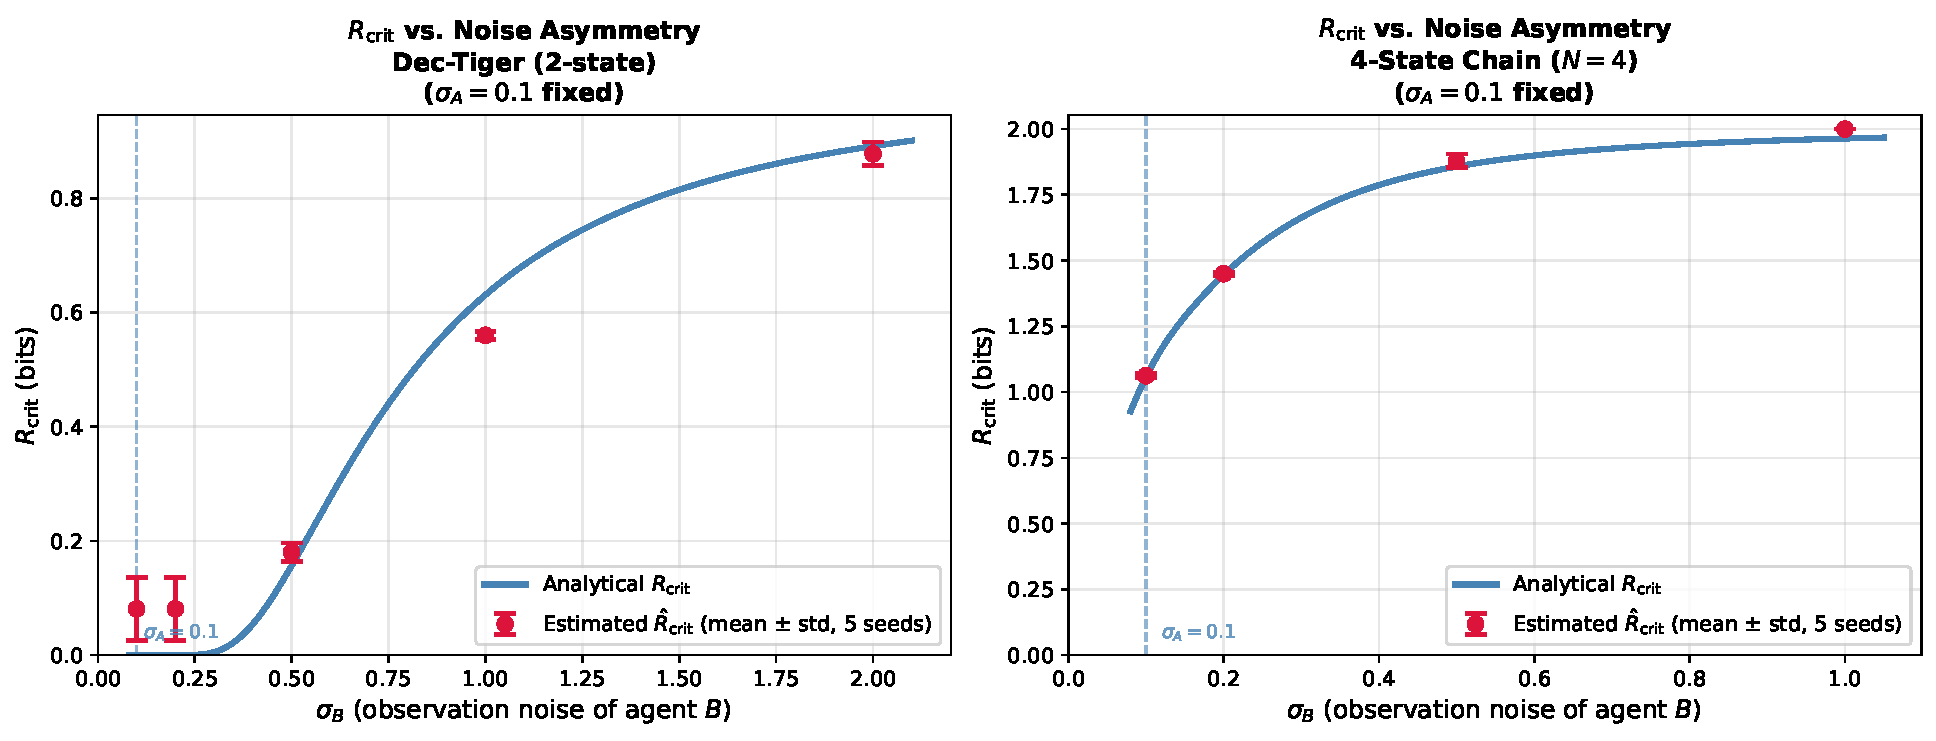
\includegraphics[width=0.90\linewidth]{rcrit_sweep.pdf}
\caption{$\hat R_{\rm crit}$ (red, mean$\pm$std over 5 seeds) vs.\ analytical
  $H(Q_A\mid Q_B)$ (blue) as $\sigma_B$ increases with $\sigma_A=0.1$.
  \emph{Left}: Dec-Tiger. \emph{Right}: 4-state chain (agent~B's quotient is
  trivial at $\sigma_B=1.0$, where the estimate is $H(\hat Q_A)=2$ bits).}
\label{fig:rcrit_sweep}
\end{figure}

% ============================================================
\section{Limitations}
\label{sec:limitations}
% ============================================================
\begin{itemize}
\item \textbf{The target is resolution-dependent.}  In continuous-observation
  POMDPs the exact history quotient is infinite; the estimator returns the
  bin-level quotient at the detection scale of the test.  Latent indices are
  recovered when $B$ is aligned with the class structure or supplied by a
  selector; over-provisioning $B$ over-splits (Table~\ref{tab:sensitivity}),
  and the PO-MuJoCo results certify separability, not a class count.
\item \textbf{One-step keys.}  All experiments use $\ell=1$; environments in
  which distinct latent classes share the same observation marginal require
  $\ell>1$ and $B^\ell$ keys, and we have not evaluated that regime.
\item \textbf{Permutation floor and multiplicity.}  With $R$ permutations no
  $p$-value is below $1/(R{+}1)$; family-wise control needs $R\gtrsim\Khist^2/\alpha$,
  and BH with all $p$-values at the floor rejects everything.  The Dec-Tiger
  over-splits are a direct consequence.
\item \textbf{Single-linkage merging.}  A single missed split merges two whole
  classes; a chain of adjacent bins with small pairwise gaps can be merged
  transitively (observed at $K=16$, $B=32$: $\hat n=12.0\pm3.1<16$).
\item \textbf{$R_{\rm crit}$ proxy.}  $H(\hat Q_A\mid\hat Q_B)$ is inflated by
  over-splitting agent~A and is a proxy for the rate of \citet{nixon2026rcrit}
  only under conditional independence of the observations given the state.
\item \textbf{Alphabet-free, not dimension-free.}  See Remark~\ref{rem:dimension}.
\end{itemize}

% ============================================================
\section{Conclusion}
\label{sec:conclusion}
% ============================================================

We extended Myhill--Nerode quotient learning to continuous observation--action
spaces by replacing the continuation G-test with a kernel-MMD permutation test
under BH control, made precise what a finite estimator can target in
continuous spaces (the bin-level quotient at the test's resolution), proved an
alphabet-free trajectory bound with explicit constants, and validated the
pipeline on ground-truth benchmarks, PO-MuJoCo and two Dec-POMDPs, reporting
every seed.  Directions: bin-count selection with statistical guarantees
(rather than silhouette), longer history keys ($\ell>1$), and a multi-agent
$R_{\rm crit}$ estimator that is robust to over-splitting.

% ============================================================
%  References
% ============================================================
\bibliographystyle{plainnat}
\bibliography{refs}

\end{document}
